% This is "sig-alternate.tex" V2.1 April 2013
% This file should be compiled with V2.5 of "sig-alternate.cls" May 2012
%
% This example file demonstrates the use of the 'sig-alternate.cls'
% V2.5 LaTeX2e document class file. It is for those submitting
% articles to ACM Conference Proceedings WHO DO NOT WISH TO
% STRICTLY ADHERE TO THE SIGS (PUBS-BOARD-ENDORSED) STYLE.
% The 'sig-alternate.cls' file will produce a similar-looking,
% albeit, 'tighter' paper resulting in, invariably, fewer pages.
%
% ----------------------------------------------------------------------------------------------------------------
% This .tex file (and associated .cls V2.5) produces:
%       1) The Permission Statement
%       2) The Conference (location) Info information
%       3) The Copyright Line with ACM data
%       4) NO page numbers
%
% as against the acm_proc_article-sp.cls file which
% DOES NOT produce 1) thru' 3) above.
%
% Using 'sig-alternate.cls' you have control, however, from within
% the source .tex file, over both the CopyrightYear
% (defaulted to 200X) and the ACM Copyright Data
% (defaulted to X-XXXXX-XX-X/XX/XX).
% e.g.
% \CopyrightYear{2007} will cause 2007 to appear in the copyright line.
% \crdata{0-12345-67-8/90/12} will cause 0-12345-67-8/90/12 to appear in the copyright line.
%
% ---------------------------------------------------------------------------------------------------------------
% This .tex source is an example which *does* use
% the .bib file (from which the .bbl file % is produced).
% REMEMBER HOWEVER: After having produced the .bbl file,
% and prior to final submission, you *NEED* to 'insert'
% your .bbl file into your source .tex file so as to provide
% ONE 'self-contained' source file.
%
% ================= IF YOU HAVE QUESTIONS =======================
% Questions regarding the SIGS styles, SIGS policies and
% procedures, Conferences etc. should be sent to
% Adrienne Griscti (griscti@acm.org)
%
% Technical questions _only_ to
% Gerald Murray (murray@hq.acm.org)
% ===============================================================
%
% For tracking purposes - this is V2.0 - May 2012

\documentclass{sig-alternate-05-2015}
\usepackage{subfigure}

\begin{document}

% Copyright
\setcopyright{acmcopyright}
%\setcopyright{acmlicensed}
%\setcopyright{rightsretained}
%\setcopyright{usgov}
%\setcopyright{usgovmixed}
%\setcopyright{cagov}
%\setcopyright{cagovmixed}


% DOI
\doi{10.475/123_4}

% ISBN
\isbn{123-4567-24-567/08/06}

%Conference

\acmPrice{\$15.00}

%
% --- Author Metadata here ---

%\CopyrightYear{2007} % Allows default copyright year (20XX) to be over-ridden - IF NEED BE.
%\crdata{0-12345-67-8/90/01}  % Allows default copyright data (0-89791-88-6/97/05) to be over-ridden - IF NEED BE.
% --- End of Author Metadata ---

\title{Final Project Report - Topic modelling for short texts using Word Embeddings
}

%
% You need the command \numberofauthors to handle the 'placement
% and alignment' of the authors beneath the title.
%
% For aesthetic reasons, we recommend 'three authors at a time'
% i.e. three 'name/affiliation blocks' be placed beneath the title.
%
% NOTE: You are NOT restricted in how many 'rows' of
% "name/affiliations" may appear. We just ask that you restrict
% the number of 'columns' to three.
%
% Because of the available 'opening page real-estate'
% we ask you to refrain from putting more than six authors
% (two rows with three columns) beneath the article title.
% More than six makes the first-page appear very cluttered indeed.
%
% Use the \alignauthor commands to handle the names
% and affiliations for an 'aesthetic maximum' of six authors.
% Add names, affiliations, addresses for
% the seventh etc. author(s) as the argument for the
% \additionalauthors command.
% These 'additional authors' will be output/set for you
% without further effort on your part as the last section in
% the body of your article BEFORE References or any Appendices.

\numberofauthors{2} %  in this sample file, there are a *total*
% of EIGHT authors. SIX appear on the 'first-page' (for formatting
% reasons) and the remaining two appear in the \additionalauthors section.
%
\author{
% You can go ahead and credit any number of authors here,
% e.g. one 'row of three' or two rows (consisting of one row of three
% and a second row of one, two or three).
%
% The command \alignauthor (no curly braces needed) should
% precede each author name, affiliation/snail-mail address and
% e-mail address. Additionally, tag each line of
% affiliation/address with \affaddr, and tag the
% e-mail address with \email.
%
% 1st. author
\alignauthor
Adit Krishnan\\
       \affaddr{Dept of CS, UIUC}\\
       \affaddr{Urbana, Illinois}\\
       \email{aditk2@illinois.edu}
% 2nd. author
\alignauthor
Aravind Sankar\\
       \affaddr{Dept of CS, UIUC}\\
       \affaddr{Urbana, Illinois}\\
       \email{asankar3@illinois.edu}
%% 3rd. author
%\alignauthor Lars Th{\o}rv{\"a}ld\titlenote{This author is the
%one who did all the really hard work.}\\
%       \affaddr{The Th{\o}rv{\"a}ld Group}\\
%       \affaddr{1 Th{\o}rv{\"a}ld Circle}\\
%       \affaddr{Hekla, Iceland}\\
%       \email{larst@affiliation.org}
%\and  % use '\and' if you need 'another row' of author names
%% 4th. author
%\alignauthor Lawrence P. Leipuner\\
%       \affaddr{Brookhaven Laboratories}\\
%       \affaddr{Brookhaven National Lab}\\
%       \affaddr{P.O. Box 5000}\\
%       \email{lleipuner@researchlabs.org}
%% 5th. author
%\alignauthor Sean Fogarty\\
%       \affaddr{NASA Ames Research Center}\\
%       \affaddr{Moffett Field}\\
%       \affaddr{California 94035}\\
%       \email{fogartys@amesres.org}
%% 6th. author
%\alignauthor Charles Palmer\\
%       \affaddr{Palmer Research Laboratories}\\
%       \affaddr{8600 Datapoint Drive}\\
%       \affaddr{San Antonio, Texas 78229}\\
%       \email{cpalmer@prl.com}
}
% There's nothing stopping you putting the seventh, eighth, etc.
% author on the opening page (as the 'third row') but we ask,
% for aesthetic reasons that you place these 'additional authors'
% in the \additional authors block, viz.
%\additionalauthors{Additional authors: John Smith (The Th{\o}rv{\"a}ld Group,
%email: {\texttt{jsmith@affiliation.org}}) and Julius P.~Kumquat
%(The Kumquat Consortium, email: {\texttt{jpkumquat@consortium.net}}).}
%\date{30 July 1999}
% Just remember to make sure that the TOTAL number of authors
% is the number that will appear on the first page PLUS the
% number that will appear in the \additionalauthors section.

\maketitle
\begin{abstract}
In many tasks involving short texts such as opinion mining or recommendation and search on social networks, it is necessary to interpret text semantically. Inferring coherent discriminative topics that appear in these texts is fundamental to this task. However, conventional probabilistic topic models such as \cite{plsa} or \cite{lda} perform poorly on collections of short texts, owing to several factors including the lack of context words, sparsity in word frequencies and co-occurrence counts, uncommon word usage (e.g. tweets/news titles), ill-formed sentences (e.g. search snippets) and topic mixture assumptions. Most short texts tend to focus on a single topic, often a large proportion of their content is related to a single semantic theme. It is thus necessary to build robust topic models that can account for the above factors. Additionally several applications require faster topic inferencing and scalability. Thus striking a balance between performance and training times is crucial.
\\[5pt]
In this report we study recent short text topic models and propose a unit topic model (UTM) exploiting pre-trained word embeddings, which attempts to address a few prominent shortcomings of previous techniques. We evaluate our model using text classification, clustering and topic coherence on two varied short text corpora.
\end{abstract}


%
% The code below should be generated by the tool at
% http://dl.acm.org/ccs.cfm

%
% End generated code
%

%
%  Use this command to print the description
%

% We no longer use \terms command
%\terms{Theory}

\keywords{Topic Model, Word Embeddings, Topic Coherence, Short Text Classification, Short Text Clustering}

\section{Introduction}
In recent years, there has been a manifold increase in the generation of short unstructured textual content on diverse platforms such as social media, RSS news feeds and online advertising. In order to effectively exploit the enormous user generated content that is present in these texts, it is necessary to develop automated algorithms that can work with them. Automatic discovery of such information and themes has been addressed effectively through topic modelling. PLSA\cite{plsa} and LDA\cite{lda} view documents as mixtures of underlying latent themes or topics which can help uncover the structure and relations of documents within a collection. Although very effective on full size documents, LDA performs poorly on short text collections. This is mainly due to the lack of availabilty of contextual co-occurences of words and lower frequency counts\cite{wang}, among other factors.
\\
\\
Two major heuristics which have been effectively applied to short texts are topic mixture relaxation and aggregation. The first heuristic assumes that a short text is drawn from a single topic. This in turn simplfies the process of inferring topics (via statistical techniques such as Gibbs sampling). Sparsity still persists, although partly alleviated since cross topic co-occurrence counts within a document are not required. Dirichlet Mixture Model(DMM)\cite{dmm} adapts LDA to short texts with this relaxation. A prominent shortcoming of this heuristic is that it fails to account for short texts that contain diverse words, assigning them to a single topic hurts topic coherence.
\\
\\
The other heuristic uses meta information based ties that exist between short texts. For instance, Twitter's context information such as hashtags, authors, and location can be used to combine tweets and generate documents \cite{mehrotra}. However, it is hard to generalize such a strategy to work well with different domains and varied collections of short texts, for instance there is no meaningful meta information attached to short search snippets.
\\
\\
Our project is motivated by the success of recent work that does not enforce such strong assumptions on the nature of the text corpora, and build generic topic models. Furthermore, the availability of pre-trained word embeddings, such as the word2vec\cite{w2v} Google news embeddings and Glove\cite{glove}, can aid us improve our semantic understanding of these texts. Since these embeddings are trained on large corpora, they implicitly encode co-occurrence information that can address sparsity issues. Our technique aims to partition short texts to obtain coherent blocks of words which form a semantic unit within that text. It is then reasonable to apply a topic relaxation assumption on such semantic units rather than the original text itself, and model co-occurences of words within these units to infer coherent topics. 
\\
\\
Unlike Yan et al.'s work \cite{btm} which performs topic inference over word biterms, our model does not place a strong constraint on the structure or process of formation of units, but rather empirically builds them based on the content of that specific short text, guided by the corresponding representation in the embedding space. Experimental results based on text classification, text clustering and topic coherence over two varied datasets confirms the ability of our model to extract meaningful topics from noisy short texts, and scalabillity to large collections.

\section{Related Work}
In this section, we study recent models that learn topic representations for short texts. Domain and document independent topic learning and applications of word embeddings are of specific interest to us.
\subsection{Conventional Topic Models}
PLSA and LDA are designed to capture the implicit word co-occurrence pattern that is present in a collection of documents. These patterns are used to build topics. Thus the presence of a greater number of co-occurences leads to more reliable and representative topics being inferred. In a collection of short texts, it is not possible to obtain as many co-occurences thus leading to inferior topic inferencing, and hence poor performance on tasks that benefit from improved semantic annotation, such as classification and clustering. There have been earlier studies that attempt to improve the topic learning process using external knowledge of concepts from Wikipedia\cite{phan} or by clustering based on auxilary long texts that are obtained from a separate source\cite{jin}. High quality supervision via text corpora or external repositories may not be available in all domains.
\subsection{DMM}
The Dirichlet Mixture Model (DMM) is based on the assumption made in the mixture of unigrams model, which is that every unigram in a document is drawn from a single underlying topic. This assumption is generally reasonable and has been shown to significantly outperform any conventional topic model for short text mining in many studies \cite{btm, zhao}. Yin and Wang \cite{dmm} develop a collapsed Gibbs sampler for DMM and reveal it's effectiveness and simplicity, using tasks such as clustering.
\subsection{Aggregation based Topic Models}
An alternate strategy is to merge the constituent short texts into larger documents which can be subsequently processed using coventional topic models. In the context of twitter, application of hastag, timestamp and named entity based aggregation has been studied \cite{mehrotra, zhao}. However the dependence on suitable meta-infomation limits the generalizability of such models. Since meta data may not be available in several domains, such as search snippets and news tags, developing a generic model to study general short texts is necessary. SATM\cite{satm} attempts to make the aggregation process independent of the source of the short texts, by introducing the notion of pseudo documents, which are conceived by the soft aggregation of words across several short texts. These latent pseudo documents are assumed to be sampled in an LDA like manner and the topic assignments and pseudo documents are sampled in a mutually reinforcing manner. Clearly, results are highly dependent on the number of pseudo documents, which needs to be set in advance. Sparsity issues still exist although alleviated by now considering co-occurences of words across short texts which are aggregated into a pseudo document. The inference process is also computationally intensive which makes it hard to scale to large corpora.
\subsection{Biterm Topic Model}
BTM\cite{btm} attempts to explicitly model word co-occurence within a short text by assuming that every pair of words within a short text is sampled from a specific topic. BTM overcomes the rigidity of DMM since different biterms within a short text could be drawn from different topics, however it is rigid in the assignment of these biterms, since every pair of words is used in the inferencing of topics. Unrelated pairs of words could however hurt the topic formation. For instace, given a sample short text "machine product manufacturing company precision client service production" (drawn from the snippets dataset), biterms such as product manufacturing, machine precision etc are highly relevant. However biterms such as client machine, client precision are not meaningful and will hurt the topic formation process. Word embeddings provide us the means to prevent such biterms from consideration. 
\\
BTM also fares poorly in terms of scalability. For large corpora, millions of biterms are generated. Statistical Inferencing on such a large number of biterms is computationally infeasible. One of our goals is to improve cohesiveness of explicit semantic units, and to reduce computational effort. Explicitly modelling every biterm is unecessary in most cases, and the performance gains are incremental when the training time is taken into account.
\subsection{Word Embedding based models}
Word Embeddings are a valuable source of implicit word co-occurence information and distributional semantics, trained a large representative document corpus. Since they encode co-occurences implicitly, they are useful to deal with sparsity problems in short text topic models. We are particularly interested in LF-DMM \cite{lfdmm} and GPU-DMM \cite{gpudmm}, which are both recently proposed topic models that employ word embeddings in the modelling process.
\\
\cite{lfdmm} replaces the usual topic word multinomial distribution with a 2 component mixture, one based on a dirichlet multinomial component (as usual), and the second based on word embeddings. Each word is assumed to be either generated from the dirichlet multinomial topic distributions, or alternately from the word embedding space. Topics are projected onto this space through the application of a log linear optimization function, which produces a vector representation of a topic. Based on a simple switch mechanism, every word is either sampled from the DM topics or based on proximity to the vector representation of a topic. The authors propose the use of a simple bernoulli switch with a preset parameter. This simplistic switch design appears to hurt performance quite a bit. Furthermore, the optimization process for topic vectors must be carried out every sampling iteration, and this makes the inferencing process very computationally intensive.
\\
\cite{gpudmm} on the other hand, attempts to build a simpler model by extending DMM. Since sparsity of related words in a short text, and irrelevance based on a few unrelated words are two primary problems in DMM, GPU aims to address this by promoting words most related to the important words in our short text. The decision to promote the most related words to a specific word, is arrived at by studying the alignment of this word to the topic that is most likely for the whole short text. A stronger alignment would mean such a word is more related to the theme of the text, and hence it can undergo promotion for the words closest to it. GPU-DMM however could bias a short text by promoting a different number of similar words for each word chosen for promotion. Much of the proposed method is highly dependent on similarity thresholds, parameters in the sampling process, and the quality of the embeddings themselves.


\begin{figure}[t!]
    \centering
    \subfigure[]{
\label{fig:Classification performance}
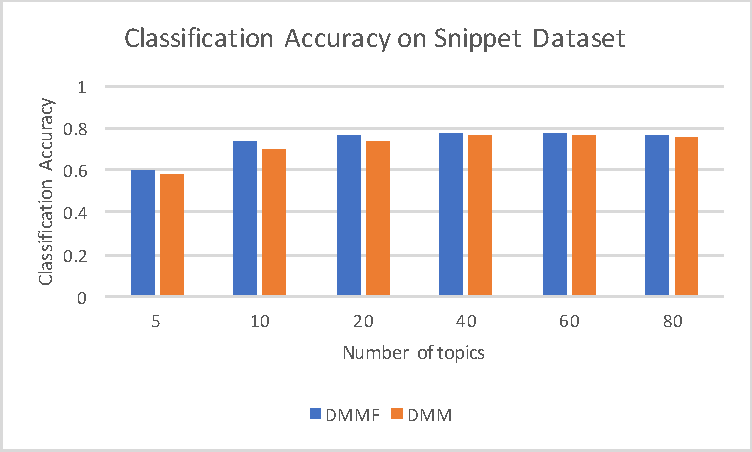
\includegraphics[width=3in]{dmmf_a.pdf}}
\subfigure[]{
\label{fig:Clustering performance}
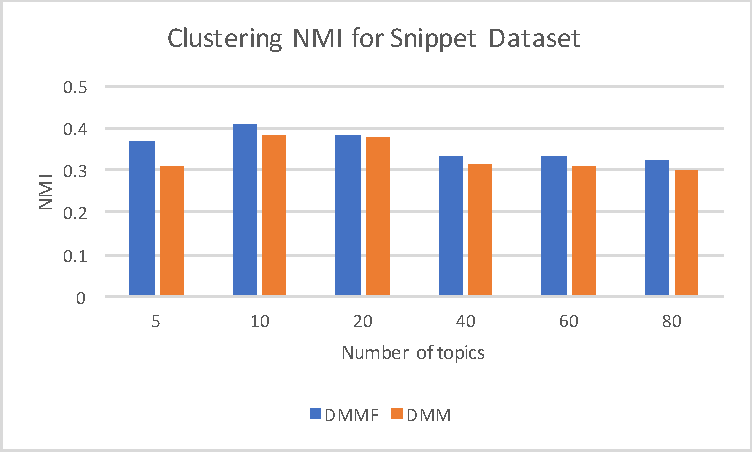
\includegraphics[width=3in]{Clustering.pdf}}
    \caption{DMM unrelated word removal}
\end{figure}

\section{Preliminary Experiments}
It is necessary to verify a few of our hypotheses with simple experiments designed to validate some of our intuitions. 
\subsection{Understanding when DMM struggles}
Although DMM proves to be a very strong contender, both in terms of simplicity and computational efficiency, as well as performance on our metrics, one of it's primary shortcomings is that irrelevant words in certain texts are often forced to be explained by topics assigned to them, which can distort the topic formation process. A simple way to verify this is to remove the most unrelated words from every short text and perform the topic modelling process on the reduced set of short texts.
\\[10pt]
More specifically, given a short text $S_{i} = {w_1, w_2 ... w_{|S_{i}|}}$, for each word $w_{j} \in S_{i}$ we define the average semantic relatedness of $w_{j}$ to $S_{i}$ as:
$$Avg.S.R(w_{j}, S_{i}) = \frac{\sum_{w_{k} \in S_{i}, k \neq j}Relatedness(w_{k}, w_{j})}{|S_{i}|-1}$$
The least semantically related words in each text are discarded (we set the value to discard several words (20\%) in order to measure it's impact on dmm results). Results were obtained from models trained before and after removal of these words for the classification and clustering tasks on the snippet dataset (We formally define the classification and clustering tasks in the experiment section), presented in \ref{fig:Classification performance} and \ref{fig:Clustering performance}.\\[10pt]
Based on inspection, it is evident that DMMF (DMM filtered) performs atleast as well as DMM (All results are averaged over 5 runs of each training cycle).
\begin{figure}[t!]
    \centering
    \subfigure[]{
\label{fig:BTM_clas}
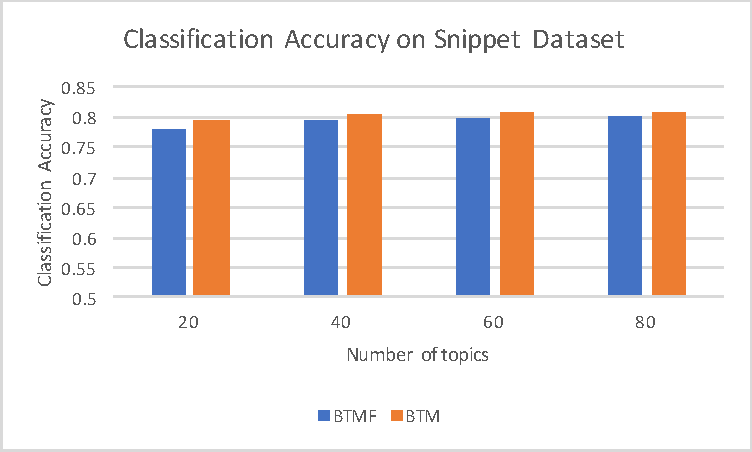
\includegraphics[width=3in]{btm_clas.pdf}}
\subfigure[]{
\label{fig:BTM_clus}
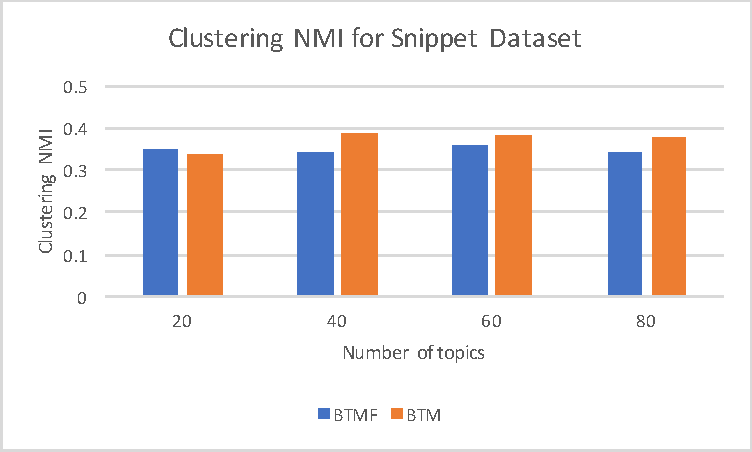
\includegraphics[width=3in]{btm_clus.pdf}}
    \caption{BTM incoherent biterm removal}
\end{figure}
\subsection{Testing our BTM hypothesis}
We hypothesize that a large proportion of BTM's word pairs are likely to be incoherent in most corpora. To test this, we remove the bottom 50\% of all biterms generated from the Snippet dataset and retrain the BTM model on this reduced set of biterms, in order to evaluate change in performance, again on the classification and clustering tasks (\ref{fig:BTM_clas} and \ref{fig:BTM_clus}). The biterms are sorted based on the cosine similarity of the constituent terms in the word2vec embedding space.
\\[5pt]
Although there is a performance drop in BTMF (BTM after filtering), given the drastic reduction in the number of biterms (by 50\%), qualitatively the drop appears to be marginal.

\section{Unit Topic Model}
\subsection{Unit Generative Model}
In this section we define out topic model, UTM. UTM requires input in the form of a set of units, which are partitions of the short texts present in the corpora. In this project we separate the process of unit formation from that of topic inferencing in UTM. As a future extension, we intend to look at a joint generative process that simultaneously learns unit partitions and topics.
\\
\begin{figure}
\label{UTM}
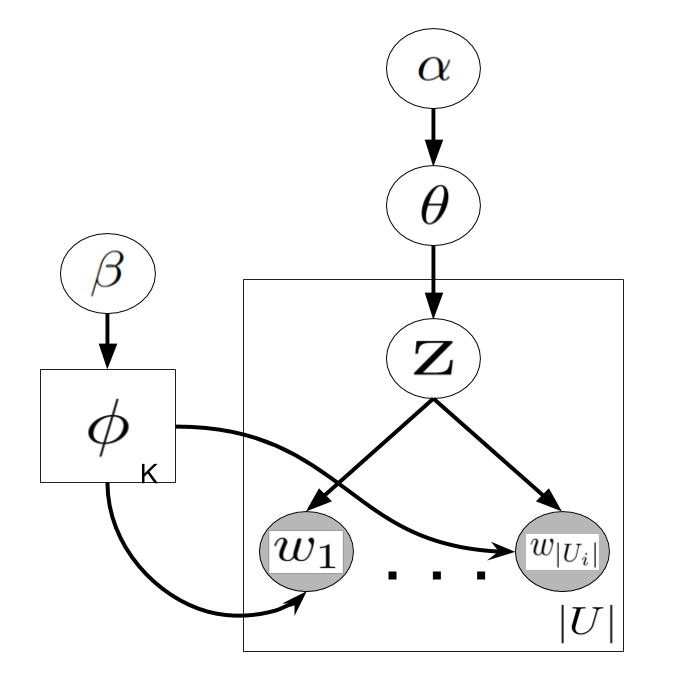
\includegraphics[width=3in]{utm}
\end{figure}
The UTM models assumes that topic proportions and topic word distributions are drawn from a dirichlet prior, similar to LDA. However since each unit is assumed to be drawn from a single topic, there is a single global topic proportion. All the words in a unit are drawn from the same topic, according to the dirichlet multinomial topic word distribution. The generative process is as follows:
\begin{itemize}
\item Sample a global topic proportion $\theta \; \sim \; Dirichlet(\alpha)$
\item For each topic k $\in {1, ... ,K}:$ \begin{itemize} \item[] Draw a topic-word distribution $\phi_{k} \; \sim \; Dirichlet(\beta)$\end{itemize}
\item For each unit $U_{i} \in U$\begin{itemize}
\item[a] Sample a topic $z_{i} \; \sim \; Multinomial(\theta)$ 
\item[b] For each word w $\in U_{i}$: \begin{itemize} \item[] Sample w $\sim \; Multinomial(\phi_{z_{i}})$\end{itemize}
\end{itemize}
\end{itemize}
\ref{utm} illustrates the above process. Inferencing is carried out via Gibbs sampling. Details are provided in the Experiments section.
%ACKNOWLEDGMENTS are optional
\subsection{Inference by Gibbs Sampling}
In this section, we define the procedure to obtain parameters $\phi$ and $\theta$ in UTM. Similar to LDA, exact inferencing of topics and topic proportion is computationally intractable. Thus it is necessary to apply an approximate inferencing algorithm. Gibbs sampling is a widely used MCMC algorithm, which has the advantages of asymptotically approaching the correct distribution as the number of iterations performed is increased, and can be memory efficient since it only needs to store the current states of units, and the word-topic assignment counts. In our system, we condition the topic distribution for a single unit, based on the current states of all other units, and sample a new topic assignment from the corresponding conditional distribution.
\\[10pt]
We begin by choosing initial states randomly for all units, and subsequently calculate the conditional distribution given by $$P(z | z_{\neg U _{i}}, U, \alpha, \beta)$$  where U is the pre defined set of all units in our short text corpus, $z_{\neg U_{i}}$ is the set of topic assignments for all the remaining units except the $i^{th}$ unit for which a topic assignment is currently being sampled and $\alpha$ and $\beta$ are the topic proportion and word-topic distribution priors, respectively. This can be given by:
\[ P(z=k \mid z_{-u} , U, \alpha, \beta) = \frac{n_{k, \neg d} + \alpha}{U-1 + K \alpha} \times \frac{\prod\limits_{w \in u} n^w_{k, \neg d} + \beta }{\prod\limits_{w \in u} n_{k, \neg d} + V \beta} \]
\begin{align*}
& n^w_{k, \neg d} : \text{Number of times word w is assigned to topic k} \\
& n_{k, \neg d} : \text{Number of units assigned to topic k} \\
\end{align*}
Intuitively this is fairly easy to interpret. The first term in the probability computation counts the number of units assigned to the current topic, smoothed by the dirichlet prior $\alpha$. The second term is a product over the probabilities of each word in this unit being assigned to topic z, smoothed by dirichlet prior $\beta$. Similarly we update the word-topic distribution and topic probabilities: \\
$$\phi_{z}(w) = \frac{n^w_{k} + \beta}{\sum_{w}{n^w_k} + M\beta}$$
$$\theta_{z} = \frac{n_{z} + \alpha}{U-1 + K\alpha}$$
For the sake of brevity, we omit the detailed derivation of this sampler.

\subsection{Semantic Enrichment/Expansion of Short Texts}
Given a short text $S_{i}$ = ${w_{1},w_{2} ... w_{|S_{i}|}}$, our goal is to discover a partition U = ${U_{1}, U_{2} ... U_{u(S_{i})}}$ of $S_{i}$ such that $$\cup_{u=1}^{u(S_{i})}U_{u} = \mathbf{S_{i}}$$ where $u(S_{i})$ is the total number of semantically diverse units chosen for the $i^{th}$  short text and, $$\mathbf{S_{i}} = S_{i} \cup E(S_{i})$$ where $E(S_{i})$ is a set of related words that is appended to $S_{i}$ based on co-occurrence knowledge (distributional semantic information). The addition of $E_{i}$ enriches the content of $S_{i}$ and helps obtain better units upon partitioning it.
\\
\\
There are 2 sources of distributional semantics that we apply to split our short texts and to discover closely related words that can be appended to our text to produce better units and deal with sparsity. The first source is the set of pre-trained 300 dimensional word2vec embeddings. Since this is trained on a very vast external corpus, we call this our global co-occurrence information.\\ On the other hand, there is information hnidden in the current corpus of short texts that we are working with. This local co-occurrence information can be captured by running a coarse DMM (low topic count) model on the corpus which involves minimal computation. This returns us a word-topic vector for every word in the corpus (we denote this vector as $v_{cDMM}(w_{j}) = \{p_{cDMM}(z|w_{j}), z \in \{1 ... K\}\}$). This also helps us deal with words that are not present in our embeddings vocabulary.
\subsubsection{Word Promotion}
In order to deal with sparsity problems and form coherent unit partitions, we extend our input short texts using semantically related words that can enhance the dominant semantic theme of a short text. We do this by choosing a set of words within each short text, that are 'promoted'. Promotion here refers to the process of increasing their semantic influence by adding words that are closely related to these promoted words in the embedding space, to the short text. The process of deciding which words to promote is based on the cDMM vectors that we mentioned earlier. The cDMM vectors let us know how likely it is that a specific word is aligned to the overall semantic theme of this short text. The higher the alignment, the more likely it is that we promote this word.\\
We model the topical alignment of a short text S as follows:
$$P(z=k|S) \propto P(z=k)\times \pi_{i=1}^{N_S} P(w_{i}|z=k)$$
where S is the short text in consideration, and $P(w|k)$ and $P(z=k)$ are obtained from the counts in the final iteration of training of cDMM on the corpus. The above probability is based on the Sum over Words (SW) formulation which is frequently applied in the context of short text classification \cite{btm}. \\
Similarly word alignment information is available in the form of $P(z=k|w)$ which can also be inferred from the assignments in the final iteration of cDMM training. Thus we obtain K-dimensional topical alignment vectors for the short text as well as it's words (we denote them as $A_{S}$ and $A_{w}, w \in S$ respectively. We then measure the likelihood that the word w is part of the semantic theme of short text S in terms of the similarity of their alignment vectors. The higher the similarity the more likely it is that we promote word w by adding it's closest semantic neighbors in the embedding space.
$$P(\text{w is promoted}) \propto Similarity(A_{S}, A_{w})$$
In our experiments we use the cosine similarity function in the above equation. A coin loaded with the above probability is then flipped to decide if a word in S is promoted or not.
\subsubsection{Semantic Expansion}
For every word that is chosen to be promoted a maximum of 5 words are added to the short text. A threshold value $\tau$ is set to the cosine similarity values, based on inspection of several common words and all their related words in the embedding space. An exception to this is when words have too many related words. For instance, names of countries often link to other countries' names with a very high cosine similarity. However this does not make them strongly semantically related. We do not promote any such words, which have a very high number of words crossing the threshold value. The expansion set E is thus constructed as follows:
$$E(S_{i}) = \{w; w \notin S_{i}, \exists w'\in S_{i}\; s.t \; sim(w, w') > \tau\}$$
$$\mathbf{S_{i}} = S_{i} \cup E(S_{i})$$
\subsection{Partioning into Units}
We implement and report experimental results for two differnt partioning schemes that appear to perform effectively. Although we experimented with several sophisticated partioning schemes, which increase computational overheads, performance gains were marginal. We describe a few of these schemes as well.
\subsubsection{K-Means based partitioning}
For every short text $S_{i}$, the corresponding expanded short text $\mathbf{S_{i}}$ is projected onto the word2vec 300 dimensional embedding space. A k-means clustering algorithm is then applied to detect clusters of related embeddings from $S_{i}$. The choice of number of clusters is decided by the ratio of average intra cluster to inter cluster L2 distances, and alternately using average intra cluster cohesiveness (which can be defined as the average mutual similarity of words within clusters, averaged across all clusters). For our experiments we use the cohesiveness metric to decide the value of k, the number of clusters/units.
\subsubsection{K-medoids based on Linear Partioning Metric}
The previous partioning metric is purely based the word2vec embedding space representation of the contents of each short text. It might be beneficial to include co-occurence information based on our own corpus as well, in addition to that provided by the GoogleNews corpus. In order to address this, we propose a simple pairwise linear similarity metric(LSM) between a pair of words in a given short text.
\\
\begin{align*}
LSM(w_{i}, w_{j}) &= \lambda \times sim(v_{cDMM}(w_{i}), v_{cDMM}(w_{j})) \\
&+ (1-\lambda) \times sim(\bar{w_{i}}, \bar{w_{j}})
\end{align*}
where $\lambda$ is an empirical weight and $\bar{w}$ represents the word2vec vector representation of word w.
\\
Given the pairwise similarity/distance for every pair of words within a given short text $\mathbf{S_{i}}$, we can now perform k-medoids based clustering on these words to obtain units. The number of clusters, i.e. k, is set in a manner similar to the previous partitioning scheme.
\subsubsection{Overlapping Probabilistic Unit Formation}
The above two partioning methods produce non overlapping units. However, in some cases generation of overlapping units might be beneficial when some words fit in well into multiple topics due to their mutual semantic relations with other words in these topics. We propose a simple probabilistic unit formation method.
\begin{itemize}
\item[] For every word $w \in S$, choose to promote w with a probability proportional to the topical alignment of w with S (as defined section 4.3.1). 
\item If a word w is promoted, a new unit is constructed, $u_{w}$. The word w is added to this unit. Now: \begin{itemize}
\item For every w' $\in$ S and w' $\neq$ w, flip a loaded coin with probability proportional to the average cosine similarity of w' to every other word that is present in the new unit $u_{w}$.
\item If the coin flip is successful add w' to $u_{w}$ and proceed to next word w''.
\end{itemize}
Overlapping topic formation tends to perform relativ ely poor. We deduce two primary reasons for this. Firstly most cosine similarities of common word pairs lie in a very small range of values between 0.4 to 0.6 in the word2vec embedding space. This causes practically every word to be promoted with a constant probability of 0.5 which is similar to random promotion. Secondly, some words could be left out in the above process if they are not successfully introduced into any unit. These two effects of random selection are quite hard to deal with in an unbiased manner.
\end{itemize}
\begin{center}
\begin{table}[t]
\label{ta1}
\begin{tabular}{c|cccc}
\hline
Dataset & \# Docs & Avg. Len & \# Labels & Vocab\\
\hline
Snippet & 12340 & 10.72 & 8 & 5977\\
\hline
 TMN & 32503 & 4.9 & 7 & 8173\\
\hline
\end{tabular}
\caption{Dataset Description}
\end{table}
\end{center}
\section{Evaluation}
\subsection{Dataset Description}
We work with 2 short text dataset that are obtained from very varied sources. Both datasets\footnote{http://acube.di.unipi.it/tmn-dataset/} are publicly available for download. The details are as tabulated in Table 1.

\subsection{Experimental Setup}
We implement Gibbs Sampling inferencing algorithms with priors $\alpha$ set to $\frac{50}{K}$ where K is the number of topics (set between 20-80 in most experiments for both datasets), $\beta$ set to 0.01 (\cite{btm,dmm}) and number of Gibbs Iterations set to 1000. Additionally threshold $\tau$ for semantic expansion is set to 0.5, linear similarity proportion $\lambda$ is set to 0.5, and coarse DMM run with K set to 5 topics.

\subsection{Evaluation Metrics}
We evaluate performance on 3 common tasks in the context of short text topic models, namely Short Text Classification, Short Text Clustering and Topic Coherence. Classification and Clustering are evaluated against the respective ground truth labels that are present in the dataset. The details of the evaluation methodology are as follows:
\subsubsection{Short Text Classification} 
The results of our inferencing process provide us a topical alignment or topic distribution vector $p(z|S)$ for every short text in our corpus. Hence, an indirect assessment of the quality of topics and assignments of texts to topics, can be measured as the accuracy of a classifier that relies on the $\{p(z|S)\}$ vector to perform classification. We employ a Support Vector Machine (SVM) with linear kernel settings, and default parameters in the python sklearn package, and the accuracy of classification is determined via 5 fold cross validation on both datasets.
\\
\\
Since all the models considered here assume single topics for short documents (units), it could be inappropriate to esimate topical distributions for classification merely based on the final topic assignments \cite{gpudmm, btm}. The post inference probabilities $p(z|d)$ is generally inferred in two different ways:
\\
\textbf{Naive Bayes (NB) Rule:}
Each word appearence is independently assumed to be drawn from the topic assigned to a unit. Hence:
$$p(z=k |S) \propto p(z=k)/;\pi_{i=1}^{N_{S}}p(w_{i}|z=k)$$
\\
\textbf{Summation over Words (SW) Rule:}
Every word in the vocabulary is used to establish the likelihood of a topic given a document using chain rule.
$$p(z=k |S) \propto \sum_{w}p(z=k|w)p(w|d)$$
Although there is no study thoroughly evaluating the relative performance of the NB and SW methods for classification, \cite{satm} shows the SW approach to largely improve classification results with DMM and LDA based topics. All of our experimental results employ SW based classification.

\subsubsection{Short Text Clustering} 
There are two simple ways to cluster text based on the inferencing results that we obtain. The first it to assign each short text S to the z which maximizes probabability of assignment:
$$z_{S} = argmax_{z \in \{1, ... ,K\}}p(z|S)$$
This produces between 1 and K clusters, where K is the total number of topics. An alternate assignment strategy is to run K-means on the $\bar{p(z|S)}$ vectors. We leave this for future work, and currently perform clustering using the max assignment. Our clusters are evaluated using the NMI (Normalized Mutual Information) metric.
\\

\begin{align*}
NMI(\Omega, \mathbb{C)} &= \frac{I(\Omega ; \mathbb{C})}{\left[ H(\Omega) + H (\mathbb{C} \right] /2} \\[5pt]
&= \frac{ \sum_{i, j} \frac{| \omega_i \cap c_j|}{n} \log \frac{|\omega_i| |c_j|}
{n |\omega_i \cap c_j|} }{(\sum_i \frac{|\omega_i|}{n} \log \frac{\omega_i}{n} + \sum_j \frac{|c_j|}{n} \log \frac{c_j}{n})/2}
\end{align*}
NMI penalizes the mutual information of clusters, $I(\Omega ; \mathbb{C})$ by their entropies in order to avoid bias towards a large number of clusters. It equals 1 if the 2 clusters are a perfect match, and lies between 0 and 1 in all other scenarios.
\subsubsection{Topic Coherence}
Topic Coherence attempts to capture the semantic cohesiveness of the topics built by the inferencing process. Words that appear in the top T spots of a topic, must be semantically related in order for the topic to be meaningful. We measure the semantic coherence of the top words of each topic, by applying cosine similarity to the corresponding Glove - 50 dimensional pre trained embeddings. This is an unbiased way to evaluate topic coherence, since word2vec and Glove embeddings are trained on different corpora and are obtained by optimizing different functions.
\\
Thus given the set of K topics, we choose the top T words for each topic, ranked by $p(w|z)$, and compute their average cosine similarity.
$$Topic \;Coherence = \frac{1}{K \times ^{T}C_{2}}\sum_{k}\sum_{1 \leq i < j \leq T}sim(w_{i}, w_{j})$$

\subsubsection{Results and Interpretation}
\begin{figure}[t!]
    \centering
    \subfigure[]{
\label{fig:Classi performance}
\includegraphics[width=3in]{images/Class_snip.pdf}}
\subfigure[]{
\label{fig:Classitmn performance}
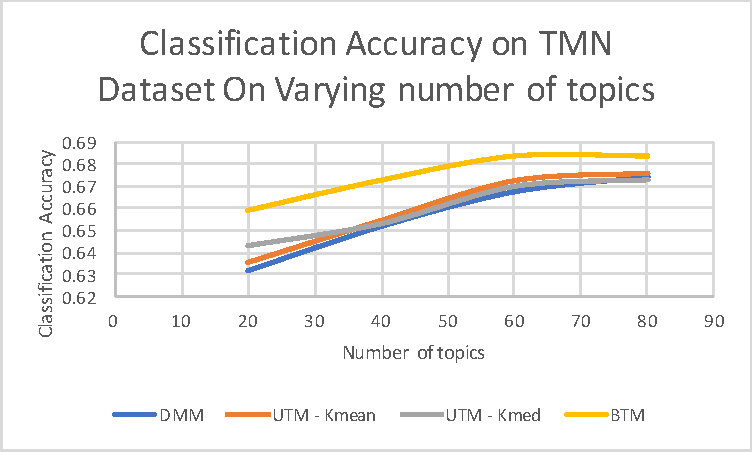
\includegraphics[width=3in]{images/Class_TMN.pdf}}
    \caption{Classification Performance}
\end{figure}
Figure 3 reports classification performance of BTM, DMM and our 2 methods on both the datasets. BTM outperforms other methods by a significant margin. UTM K-mean and UTM K-med perform similar to DMM, although UTM K-Mean does marginally better.
\\[5pt]
Figure 4 reports clustering performance measured by NMI, for the same set of methods. UTM K-Mean and BTM outperform DMM by a significant margin.
\\[5pt]
Figure 5 reports topic coherence in our methods vs DMM and BTM. Our methods can be seen to be atleast comparable or better than BTM in this metric. A possible reason for this, is that BTM overfits to the dataset that it is trained on. This causes it to perform very well on the classification and clustering tasks, but not as well on topic coherence evaluated against an external source. 
\\[5pt]
Figure 6 reports the runtime per iteration of all 4 algorithms. Our runtimes can be seen to be comparable with DMM. BTM on the other hand is significantly slower and scales poorly as the number of topics or the size of the corpus is increased. This causes BTM to be computationally infeasible for most real world applications involving millions of text snippets. 
\begin{figure}[t!]
    \centering
    \subfigure[]{
\label{fig:Clus performance}
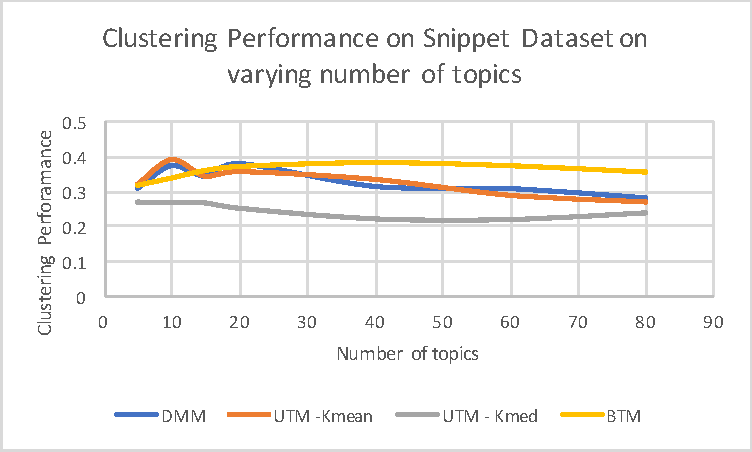
\includegraphics[width=3in]{images/Clus_Snip.pdf}}
\subfigure[]{
\label{fig:Clustmn performance}
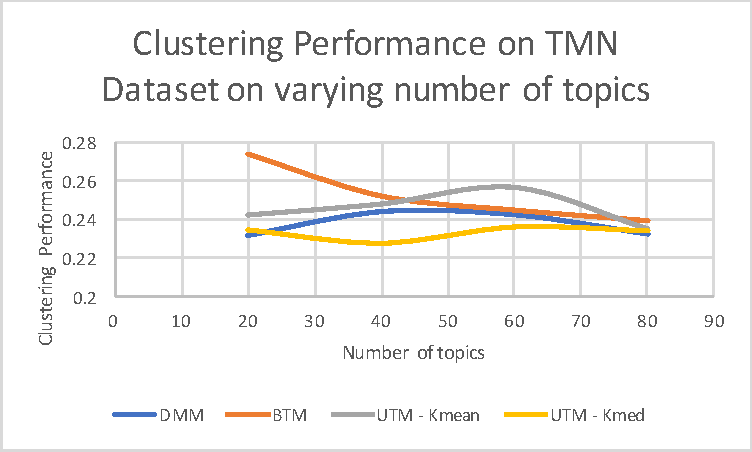
\includegraphics[width=3in]{images/Clus_TMN.pdf}}
    \caption{Clustering Performance (NMI)}
\end{figure}
\begin{figure}[t!]
    \centering
    \subfigure[]{
\label{fig:TC performance}
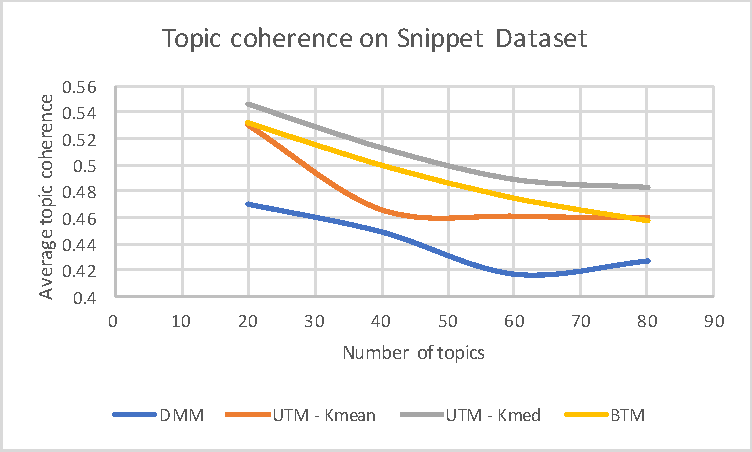
\includegraphics[width=3in]{images/TC_Snip.pdf}}
\subfigure[]{
\label{fig:TCtmn performance}
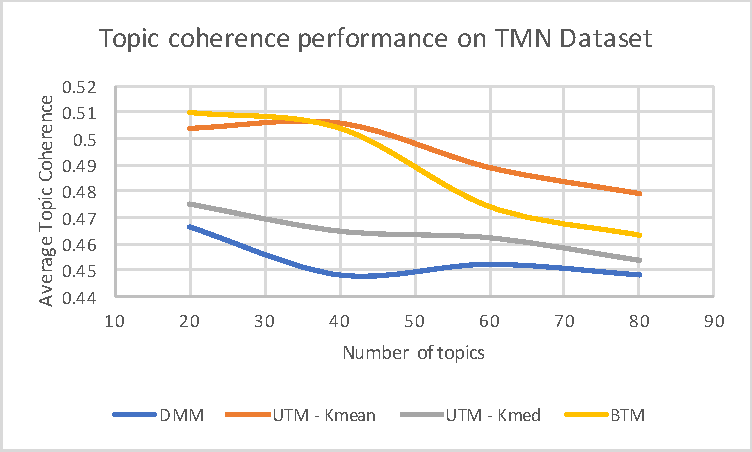
\includegraphics[width=3in]{images/TC_TMN.pdf}}
    \caption{Topic Coherence}
\end{figure}
\begin{figure}[t!]
    \centering
    \subfigure[]{
\label{fig:TC performance}
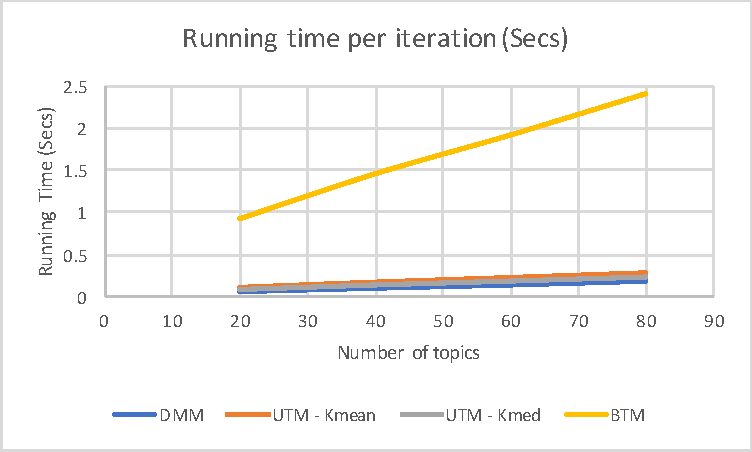
\includegraphics[width=3in]{images/Time_Snip.pdf}}
\subfigure[]{
\label{fig:TCtmn performance}
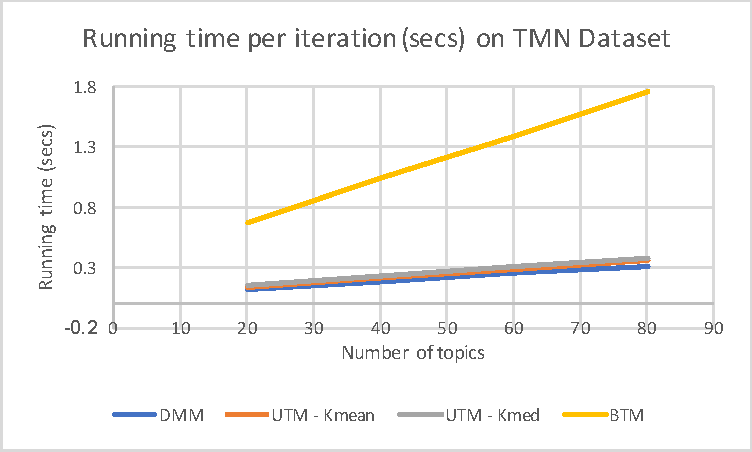
\includegraphics[width=3in]{images/Time_TMN.pdf}}
    \caption{Runtime per Gibbs iteration}
\end{figure}
%
% The following two commands are all you need in the
% initial runs of your .tex file to
% produce the bibliography for the citations in your paper.
\bibliographystyle{abbrv}
\bibliography{sigproc}  % sigproc.bib is the name of the Bibliography in this case
% You must have a proper ".bib" file
%  and remember to run:
% latex bibtex latex latex
% to resolve all references
%
% ACM needs 'a single self-contained file'!
%
%APPENDICES are optional
%\balancecolumns

%Appendix A



%Generated by bibtex from your ~.bib file.  Run latex,
%then bibtex, then latex twice (to resolve references)
%to create the ~.bbl file.  Insert that ~.bbl file into
%the .tex source file and comment out
%the command \texttt{{\char'134}thebibliography}.
% This next section command marks the start of
% Appendix B, and does not continue the present hierarchy



\end{document}
